% \chapter{Wstęp} masterPage
% \section{Zakres}
\subsection{Front-end}
\begin{itemize}
	\item Konsolowy interfejs użytkownika umożliwiający wydawanie komend do:
	\begin{itemize}
		\item Kontrolera sterownika;
		\item Bazy danych;
	\end{itemize}
	\item Realizacja wzorców projektowych:
	\begin{itemize}
		\item Komenda;
		\item Metoda szablonowa;
	\end{itemize}
	\item Przekazywanie logów aplikacji z Back-endu;
	\item Walidacja komend wpisanych przez użytkownika:
	\begin{itemize}
		\item Odrzucanie nieznanych komend;
		\item Podpowiedź odnośnie wartości argumentów komend już znanych;
	\end{itemize}
\end{itemize}

\begin{figure}[h!]
    \centering
    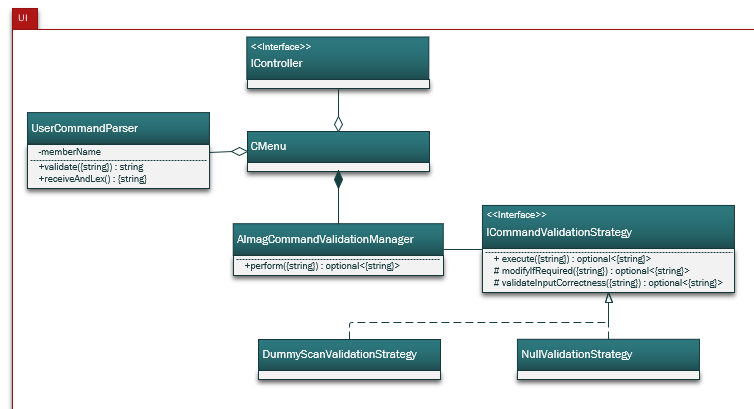
\includegraphics[scale=0.90]{Obrazki/DiagramyKlas/UI.png}
    \caption{Diagram klas przedstawiający klasy wchodzące w skład interfejsu użytkownika.
        \newline(Opracowanie własne)}
\end{figure}

\subsection{Testowanie}
\begin{itemize}
\item Front-end
	\begin{itemize}
		\item Jednostkowe
		\item Modułowe
	\end{itemize}
\item Back-end
	\begin{itemize}
		\item Jednostkowe
		\begin{itemize}
			\item HDLC
			\item HDLC Body
			\item DB
		\end{itemize}
		\item Modułowe
		\begin{itemize}
			\item Happy Path
			\item Sad Path
		\end{itemize}
		\item Integracja
		\begin{itemize}
			\item UI + DB
			\item UI + DB + Back-end Controller
		\end{itemize}
	\end{itemize}
\item Komponentowe \newline
	W celu weryfikacji działania symulatora sterownika od początku do końca zalecane jest uruchomienie całego komponentu 
	jako czarną czarną skrzynkę oraz operowanie na nim przy pomocy zaimplementowanego interfejsu. W tym celu
	zaimplementowany został również symulator urządzenia, który odbiera wiadomości oraz odpowiada na nie.
\end{itemize}
